        %%******************************************%%
        %%                                          %%
        %%        Modello di tesi di laurea         %%
        %%            di Andrea Giraldin            %%
        %%                                          %%
        %%             2 novembre 2012              %%
        %%                                          %%
        %%******************************************%%

\begin{document}
    \frontmatter
    \begin{titlepage}
    \begin{center}
        \begin{LARGE}
            \textbf{\myUni}\\
        \end{LARGE}

        \vspace{10pt}

        \begin{Large}
            \textsc{\myDepartment}\\
        \end{Large}

        \vspace{10pt}

        \begin{large}
            \textsc{\myFaculty}\\
        \end{large}

        \vspace{30pt}
        \begin{figure}[htbp]
            \centering
            
\includegraphics[height=6cm]{unipd-logo}
        \end{figure}
        \vspace{30pt}

        \begin{LARGE}
            \textbf{\myTitle}\\
        \end{LARGE}

        \vspace{10pt}

        \begin{large}
            \textsl{\myDegree}\\
        \end{large}

        \vspace{40pt}

        \begin{large}
            \begin{flushleft}
                \textit{Relatore}\\
                \vspace{5pt}
                \profTitle\ \myProf
            \end{flushleft}

            % You can tweak the spacing to have professor and student names on the same line
            % useful if the page is broken by a long thesis title and you need more space
            % \vspace{-52pt}

            \begin{flushright}
                \textit{Laureando}\\
                \vspace{5pt}
                \myName
            \end{flushright}
        \end{large}

        \vspace{40pt}

        \line(1, 0){338} \\
        \begin{normalsize}
            \textsc{Anno Accademico \myAA}
        \end{normalsize}
    \end{center}
\end{titlepage}

    \clearpage
\phantomsection
\thispagestyle{empty}

\hfill
\vfill

\noindent\myName: \textit{\myTitle,}
\myDegree,
\textcopyright\ \myTime.

    \cleardoublepage
\phantomsection
\thispagestyle{empty}
\pdfbookmark{Dedica}{Dedica}

\vspace*{3cm}

\begin{center}
    Lorem ipsum dolor sit amet, consectetuer adipiscing elit. \\ \medskip
    --- Oscar Wilde
\end{center}

\medskip

\begin{center}
    Dedicato a ...
\end{center}

    \cleardoublepage
\phantomsection
\pdfbookmark{Sommario}{Sommario}
\begingroup
\let\clearpage\relax
\let\cleardoublepage\relax
\let\cleardoublepage\relax

\chapter*{Sommario}

Il presente documento descrive il lavoro svolto durante il periodo di stage, della durata di circa trecento ore, dal laureando Pinco Pallino presso l'azienda Azienda S.p.A.
Gli obbiettivi da raggiungere erano molteplici.\\
In primo luogo era richiesto lo sviluppo di ...
In secondo luogo era richiesta l'implementazione di un ...
Tale framework permette di registrare gli eventi di un controllore programmabile, quali segnali applicati
Terzo ed ultimo obbiettivo era l'integrazione ...

%\vfill

%\selectlanguage{english}
%\pdfbookmark{Abstract}{Abstract}
%\chapter*{Abstract}

%\selectlanguage{italian}

\endgroup

\vfill

    \cleardoublepage
\phantomsection
\pdfbookmark{Ringraziamenti}{ringraziamenti}

\begin{flushright}{
    \slshape
    ``Life is really simple, but we insist on making it complicated''} \\
    \medskip
    --- Confucius
\end{flushright}


\bigskip

\begingroup
\let\clearpage\relax
\let\cleardoublepage\relax
\let\cleardoublepage\relax

\chapter*{Ringraziamenti}

%\noindent \textit{Innanzitutto, vorrei esprimere la mia gratitudine al Prof. \myProf, relatore della mia tesi, per l'aiuto e il sostegno fornitomi durante la stesura del lavoro.}\\
%
%\noindent \textit{Desidero ringraziare con affetto i miei genitori per il sostegno, il grande aiuto e per essermi stati vicini in ogni momento durante gli anni di studio.}\\
%
%\noindent \textit{Ho desiderio di ringraziare poi i miei amici per tutti i bellissimi anni passati insieme e le mille avventure vissute.}\\
\bigskip

%\noindent\textit{\myLocation, \myTime}
\hfill Erica Cavaliere

\endgroup

    \cleardoublepage
\pdfbookmark{\contentsname}{tableofcontents}
\setcounter{tocdepth}{2}
\tableofcontents
%\markboth{\contentsname}{\contentsname}
\clearpage

\begingroup
    \let\clearpage\relax
    \let\cleardoublepage\relax
    \let\cleardoublepage\relax

    % Figures list
    \phantomsection
    \pdfbookmark{\listfigurename}{lof}
    \listoffigures

    \vspace*{8ex}

    % Tables list
    \phantomsection
    \pdfbookmark{\listtablename}{lot}
    \listoftables

    \vspace*{8ex}
\endgroup

\cleardoublepage

    \cleardoublepage

    \mainmatter
    \chapter{Introduzione}
\label{cap:introduzione}

%Introduzione al contesto applicativo.\\
%
%\noindent Esempio di utilizzo di un termine nel glossario \\
%\gls{api}. \\
%
%\noindent Esempio di citazione in linea \\
%\cite{site:agile-manifesto}. \\
%
%\noindent Esempio di citazione nel pie' di pagina \\
%citazione\footcite{womak:lean-thinking} \\

\section{L'azienda}

RiskApp S.r.l. (Figura \ref{fig:riskapp}) è un'azienda con sede a Conselve (PD) che si occupa di sviluppo software per il mondo assicurativo.\newline
È stata fondata nel 2016 e il suo \textit{core business} è lo sviluppo e il mantenimento dell'omonima applicazione, che viene costantemente aggiornata ed estesa per garantire un prodotto che possa rispondere ad ogni esigenza.\newline
Il principale punto di forza di questa piattaforma è quello di stimare le possibili perdite economiche di un’impresa attraverso un algoritmo proprietario che, anche attraverso l’uso dell'intelligenza artificiale, valuta il rischio raccogliendo e combinando una moltitudine di dati da diverse fonti.\newline
Il personale aziendale lavora costantemente per migliorare i propri servizi, ragionando sui possibili problemi che l'utente e l'aziende possono andare incontro, fanno riunioni e call per capire come migliorare e ampliare la piattaforma, tutto svolto in un clima di calma e rispetto tra colleghi.

\begin{figure}[!h] 
    \centering 
    
\includegraphics[width=0.4\columnwidth]{RiskAPP} 
    \caption{Logo dell'azienda RiskApp}\label{fig:riskapp}
\end{figure}

\section{L'idea}

Per poter gestire le spese per i pasti, che preparano in azienda, è stato scelto di sviluppare un'app mobile che permetta di monitorare i versamenti degli utenti, scegliere il piatto del giorno da un menu condiviso e monitorare la \emph{\gls{cassacomuneg}}\glsfirstoccur.\newline
Deve essere gestita l'autenticazione di ogni utente, dividendo tra utente semplice e utente amministratore e permettere il controllo delle presenze in azienda durante i pranzi. \newline
Ogni utente potrà aggiungere un piatto nel menu, proporre il pasto del giorno, monitorare la sua \emph{\gls{quotastornatag}}\glsfirstoccur e la cassa comune, indicare le spese effettuate e modificare i dati personali. \newline
L'amministratore potrà anche gestire le presenze e le spese effettuate dagli stagisti.
L'applicazione dovrà essere sviluppata con \emph{\gls{flutterg}}\glsfirstoccur, \emph{\gls{dartg}}\glsfirstoccur  e \emph{\gls{firebaseg}}\glsfirstoccur.

%da modificare - vedere alla fine ----------------------------------------------------------
\section{Organizzazione del testo}

\begin{description}
    \item[{\hyperref[cap:processi-metodologie]{Il secondo capitolo}}] descrive in che modo è stato creato il prodotto desiderato, quale metodo di sviluppo è stato utilizzato e quali sono le tecnologie adottate per lavorare al progetto.
    
    %\item[{\hyperref[cap:descrizione-stage]{Il terzo capitolo}}] approfondisce ...
    
    \item[{\hyperref[cap:analisi-requisiti]{Il terzo capitolo}}] approfondisce i requisiti con una analisi dettagliata di cosa è stato richiesto.
    
    \item[{\hyperref[cap:progettazione-codifica]{Il quarto capitolo}}] approfondisce la progettazione, i \emph{design pattern} utilizzati e la struttura del codice.
    
    %\item[{\hyperref[cap:verifica-validazione]{Il quinta capitolo}}] approfondisce ...
    
    \item[{\hyperref[cap:conclusioni]{Nel quinto capitolo}}] vengono riportate le valutazioni e le conclusioni personali del prodotto.
\end{description}


%da tenere e non toccare --------------------------------------------------------------

Riguardo la stesura del testo, relativamente al documento sono state adottate le seguenti convenzioni tipografiche:
\begin{itemize}
	\item gli acronimi, le abbreviazioni e i termini ambigui o di uso non comune menzionati vengono definiti nel glossario, situato alla fine del presente documento;
	\item per la prima occorrenza dei termini riportati nel glossario viene utilizzata la seguente nomenclatura: \emph{parola}\glsfirstoccur;
	\item i termini in lingua straniera o facenti parti del gergo tecnico sono evidenziati con il carattere \emph{corsivo}.
\end{itemize}

    \chapter{Processi e metodologie}
\label{cap:processi-metodologie}

\intro{In questo capitolo viene spiegato il Material Design che sta alla base della progettazione dell'app, viene poi riportato il metodo di lavoro utilizzato e infine le tecnologie adottate per lo sviluppo del progetto.}\\

\section{Material Design}
% Nome, riscrittura senza ripetizioni del contesto (presentazione simil "marketing")
%L'applicazione è stata creata seguendo la regole di Material Design di Goggle  e i consigli di Material Components messi a disposizione da Flutter (https://docs.flutter.dev/ui/widgets/material).\newline
%Per permettere la navigazione tra le varie pagine dellàapplicazione, è stato utilizzato una barra di navigazione posta sulla lato inferiore della schermata (Figura ???)
Alla base dell'applicazione, è stato scelto di seguire il Material Design (Figura \ref{fig:material}) sviluppato da Google, che si concentra su un maggiore uso di \emph{layout} basati su una griglia, animazioni, transizioni ed effetti di profondità come l'illuminazione e le ombre.\newline
Si tratta di una serie di regole ideate per consentire una buona \emph{\gls{ux}}\glsfirstoccur e definire una \emph{\gls{ui}}\glsfirstoccur per l'utente da implementare in ambiente Web, Android e in \emph{\gls{flutterg}}.\newline
Viene annunciato per la prima volta da Google il 25 giugno del 2014 durante il Google I/O, una conferenza organizzata annualmente da Google a Mountain View, in California.\newline
\begin{figure}[!h] 
    \centering 
    
\includegraphics[width=0.2\columnwidth]{MaterialDesign} 
    \caption{Logo del Material Design di Google}\label{fig:material}
\end{figure}
\newline
Venne rinnovato nel 2018 con il Material Design 2, anche chiamato Google Material Theme, introducendo un maggiore utilizzo di angoli arrotondati, spazi bianchi e icone colorate, infine viene rinnovato nel 2021 con il Material Design 3, oppure Material You, introducendo l'uso di tasti più grandi e maggiore uso delle animazioni.\newline
Oggi viene ancora utilizzato il Material Design 3 ed è stato seguito per lo sviluppo dell'app dei pranzi.\newline
\newline
Per consentire l'uso dei propri prodotti software a più utenti possibili, il Material Design segue le regole del \emph{\gls{wcag}}\glsfirstoccur, mettendo alla base di ogni progetto l'accessibilità, creando così dei prodotti inclusivi, cioè usabili da tutti i tipi di utenti, anche con disabilità, consentendo a ciascuno un'esperienza fluida e semplice da usare.\newline
\newline
I \emph{layout} devono essere studiati in modo da guidare l'utente nella navigazione della pagina e devono essere dinamici, in modo che le pagine si adattino ad ogni tipo di schermo.\newline
Vengono indicate delle regole precise su come devono essere impostate le \emph{\gls{componentig}}\glsfirstoccur, come devono essere raggruppate, lo spazio che deve esserci e tanti altri piccoli ma importanti dettagli che lo sviluppatore deve considerare per permettere all'utente di orientarsi su qualsiasi dispositivo.\newline
Anche \emph{\gls{flutterg}} offre una guida sulle \emph{\gls{componentig}} che mette a disposizione per lo sviluppatore e che sono state ideate per rispettare le regole di Material Design appena descritte.\newline

\section{Metodo di lavoro}
Durante lo stage, RiskApp contava circa dieci dipendenti e ognuno era incaricato di sviluppare e mantenere una parte della loro piattaforma, confrontandosi tra loro ogni giorno per capire come continuare a lavorare.\newline
Il loro metodo di lavoro si avvicina a un metodo Agile, più precisamente ad uno SCRUM, utilizzato anche per lo sviluppo del progetto di stage.\newline
\newline
Il Manifesto per lo sviluppo Agile (\cite{site:manifesto-agile}) è composto da dodici principi fondamentali che descrivono il modo in cui deve lavorare il team, permettendo possibili cambiamenti in corso d'opera e mettendo al primo posto il cliente, rilasciando varie versioni del prodotto funzionante dopo brevi periodi e privilegiando le comunicazioni faccia a faccia.\newline
Lo SCRUM è un \emph{framework} di gestione dei progetti Agile che mira a cinque valori fondamentali: impegno, focus, apertura, rispetto e coraggio.\newline
Questo \emph{framework} ha acquisito negli ultimi anni una straordinaria popolarità nel mondo dell’informatica grazie ai vantaggi offerti, come maggiore collaborazione con l’utente finale, il suo contributo al miglioramento continuo e la superiore gestione dei rischi.\newline
L’idea di fondo consiste nel suddividere i periodi di lavoro in \emph{sprint} di durata fissata, caratterizzati da un insieme di obiettivi da realizzare (\emph{sprint backlog}).\newline
\newline
Per lo sviluppo del progetto di stage, ogni giorno veniva riportato quanto era stato fatto e veniva mostrato il funzionamento, raccogliendo possibili idee per migliorare o modificare l'app.\newline
Se in corso d'opera venivano incontrate eventuali problematiche sullo sviluppo, si ragionava su come affrontare o modificare il prodotto per risolvere questi problemi, permettendo così di soddisfare ogni esigenza degli utenti finali, in questo caso per soddisfare le esigenze dei dipendenti dell'azienda.

\newpage

\section{Tecnologie}

\subsection{Flutter}
Flutter (Figura \ref{fig:flutter}) è un progetto open-source di Google il cui vantaggio principale è la generazione di applicazioni multipiattaforma a partire da un unico codice sorgente.\newline
Permette quindi allo sviluppatore di concentrarsi sul prodotto da realizzare senza dover preferire un sistema operativo mobile ad un altro.\newline
Per questo motivo è stato scelto di utilizzare Flutter come \emph{framework} principale, dato che il prodotto finale deve funzionare sia per dispositivi Android sia per dispositivi iOS.\newline
\begin{figure}[!h] 
    \centering
    
\includegraphics[width=0.4\columnwidth]{Flutter} 
    \caption{Logo di Flutter}\label{fig:flutter}
\end{figure}

\subsection{Dart}
Il linguaggio sul quale si basa Flutter è Dart (Figura \ref{fig:dart}), nato con l’intento di sostituire JavaScript come protagonista delle applicazioni web.\newline
Tra i suoi pregi si elencano il compilatore JIT, migliore gestione della sicurezza, la velocità e la maggiore scalabilità.\newline
Il paradigma principale è l’orientamento agli oggetti, una sua particolarità è data dalla sua attenzione alla \emph{null safety}, per la quale nessun valore può essere nullo a meno che questa possibilità non sia esplicitamente dichiarata.\newline
\begin{figure}[!h] 
    \centering 
    
\includegraphics[width=0.4\columnwidth]{Dart} 
    \caption{Logo di Dart}\label{fig:dart}
\end{figure}

\subsection{Firebase}
Firebase (Figura \ref{fig:dart}) è una piattaforma \emph{open-source} per la creazione di applicazioni per dispositivi mobili e web sviluppata da Google.\newline
Firebase sfrutta l'infrastruttura di Google e il suo cloud per fornire una suite di strumenti per scrivere, analizzare e mantenere applicazioni \emph{cross-platform}.\newline
Infatti offre funzionalità come analisi, database (usando strutture noSQL), messaggistica e segnalazione di arresti anomali per la gestione di applicazioni web, iOS e Android.\newline
Per lo sviluppo dell'app sono stati utilizzati:
\begin{itemize}
    \item Firebase Autentication, per permettere la registrazione e l'autenticazione di un utente tramite mail e password;
    \item Cloud Firestore, per la gestione del database.
\end{itemize}
\begin{figure}[!h] 
    \centering 
    
\includegraphics[width=0.5\columnwidth]{Firebase} 
    \caption{Logo di Firebase}\label{fig:figma}
\end{figure}

\subsection{Figma}
Figma (Figura \ref{fig:figma}) è un software per la progettazione di User Interface(UI).\newline
Permette infatti di realizzare prototipi delle interfacce, detti anche \emph{mockup}, che permettono di illustrare il risultato finale che si desidera ottenere.\newline
Questo strumento è stato utilizzato per mostrare e concordare l'interfaccia dell'app al tutor aziendale, prima della fase di codifica.\newline
\begin{figure}[!h] 
    \centering 
    
\includegraphics[width=0.4\columnwidth]{Figma} 
    \caption{Logo di Figma}\label{fig:figma}
\end{figure}

\subsection{Android Studio}
Android Studio (Figura \ref{fig:android}) è un \emph{\gls{ide}}\glsfirstoccur adibito per la creazione di applicazioni Android e mette a disposizione dei simulatori virtuali di uno o più cellulari con il sistema operativo di Google.\newline
Il progetto è stato sviluppato interamente con l'uso di questo \emph{\gls{ideg}} ed è stato utilizzato il simulatore virtuale di Google Pixel 7 con sistema operativo Android 13 per testare la \emph{\gls{buildg}}\glsfirstoccur dell'app.\newline
\begin{figure}[!h] 
    \centering 
    
\includegraphics[width=0.5\columnwidth]{AndroidStudio} 
    \caption{Logo di Android Studio}\label{fig:android}
\end{figure}

\subsection{Xcode}
Xcode (Figura \ref{fig:apple}) è un \emph{\gls{ideg}} completamente sviluppato e mantenuto da Apple, contenente una suite di strumenti utili allo sviluppo di software per i sistemi macOS, iOS, iPadOS, watchOS e tvOS.\newline
Per poter testare la \emph{\gls{buildg}} del progetto, è stato utilizzato il simulatore virtuale di iPhone 15 con sistema operativo iOS 17, messo a disposizione da questo software.\newline
\begin{figure}[!h] 
    \centering 
    
\includegraphics[width=0.25\columnwidth]{Xcode} 
    \caption{Logo di Xcode}\label{fig:apple}
\end{figure}

\subsection{GitHub}
GitHub (Figura \ref{fig:github}) è una piattaforma di \emph{hosting} per per ospitare codice all'interno di repository basato sul software Git.\newline
Fornisce agli sviluppatori strumenti per migliorare e mantenere il codice come:
\begin{itemize}
    \item \emph{features} utilizzabili da linea di comando;
    \item gestione delle \emph{pull request} e \emph{code review};
    \item strumenti per l’\emph{issue tracking}.
\end{itemize}
La codebase della piattaforma RiskApp è suddivisa in varie repository su GitHub.\newline
Per questo progetto, l'azienda ha riservato una repository apposita per permettermi di lavorare in autonomia al codice.\newline
\begin{figure}[!h] 
    \centering 
    
\includegraphics[width=0.5\columnwidth]{GitHub} 
    \caption{Logo di GitHub}\label{fig:github}
\end{figure}

\newpage

\subsection{Slack}
Slack (Figura \ref{fig:slack}) è un applicazione multipiattaforma per la messaggistica istantanea tra membri di un gruppo di lavoro.\newline
Una delle funzioni di Slack è la possibilità di organizzare la comunicazione del team attraverso canali specifici, canali che possono essere accessibili a tutto il team o solo ad alcuni membri.\newline
È possibile inoltre comunicare con il team anche attraverso chat individuali private o chat con due o più membri.\newline
Questo software è stato utilizzato per comunicare con il tutor aziendale da remoto e per condividere materiale.\newline
\begin{figure}[!h] 
    \centering 
    
\includegraphics[width=0.4\columnwidth]{Slack} 
    \caption{Logo di Slack}\label{fig:slack}
\end{figure}


    \chapter{Descrizione dello stage}
\label{cap:descrizione-stage}

\intro{Breve introduzione al capitolo}\\

\section{Introduzione al progetto}

\section{Analisi preventiva dei rischi}

Durante la fase di analisi iniziale sono stati individuati alcuni possibili rischi a cui si potrà andare incontro.
Si è quindi proceduto a elaborare delle possibili soluzioni per far fronte a tali rischi.\\

\begin{risk}{Performance del simulatore hardware}
    \riskdescription{le performance del simulatore hardware e la comunicazione con questo potrebbero risultare lenti o non abbastanza buoni da causare il fallimento dei test}
    \risksolution{coinvolgimento del responsabile a capo del progetto relativo il simulatore hardware}
    \label{risk:hardware-simulator} 
\end{risk}

\section{Requisiti e obiettivi}


\section{Pianificazione}

    \chapter{Analisi dei requisiti}
\label{cap:analisi-requisiti}

\intro{Breve introduzione al capitolo}\\

\section{Casi d'uso}

Per lo studio dei casi di utilizzo del prodotto sono stati creati dei diagrammi.
I diagrammi dei casi d'uso (in inglese \emph{Use Case Diagram}) sono diagrammi di tipo \gls{uml} dedicati alla descrizione delle funzioni o servizi offerti da un sistema, così come sono percepiti e utilizzati dagli attori che interagiscono col sistema stesso.
Essendo il progetto finalizzato alla creazione di un tool per l'automazione di un processo, le interazioni da parte dell'utilizzatore devono essere ovviamente ridotte allo stretto necessario. Per questo motivo i diagrammi d'uso risultano semplici e in numero ridotto.

\begin{figure}[!h] 
    \centering 
    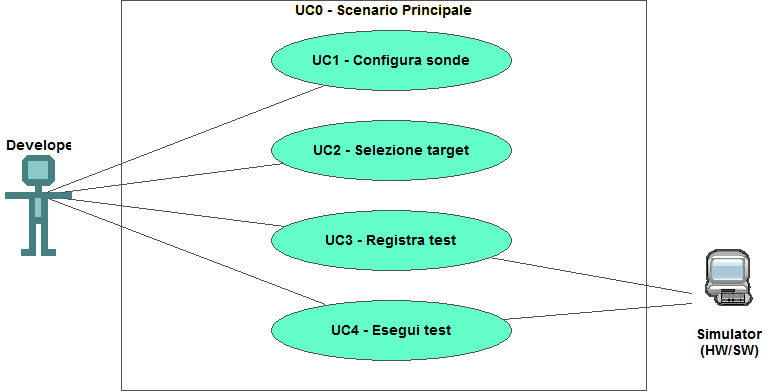
\includegraphics[width=0.9\columnwidth]{usecase/scenario-principale} 
    \caption{Use Case - UC0: Scenario principale}
\end{figure}

\begin{usecase}{0}{Scenario principale}
\usecaseactors{Sviluppatore applicativi}
\usecasepre{Lo sviluppatore è entrato nel plug-in di simulazione all'interno dell'IDE}
\usecasedesc{La finestra di simulazione mette a disposizione i comandi per configurare, registrare o eseguire un test}
\usecasepost{Il sistema è pronto per permettere una nuova interazione}
\label{uc:scenario-principale}
\end{usecase}

\section{Tracciamento dei requisiti}

Da un'attenta analisi dei requisiti e degli use case effettuata sul progetto è stata stilata la tabella che traccia i requisiti in rapporto agli use case.\\
Sono stati individuati diversi tipi di requisiti e si è quindi fatto utilizzo di un codice identificativo per distinguerli.\\
Il codice dei requisiti è così strutturato R(F/Q/V)(N/D/O) dove:
\begin{enumerate}
	\item[R =] requisito
    \item[F =] funzionale
    \item[Q =] qualitativo
    \item[V =] di vincolo
    \item[N =] obbligatorio (necessario)
    \item[D =] desiderabile
    \item[Z =] opzionale
\end{enumerate}
Nelle tabelle \ref{tab:requisiti-funzionali}, \ref{tab:requisiti-qualitativi} e \ref{tab:requisiti-vincolo} sono riassunti i requisiti e il loro tracciamento con gli use case delineati in fase di analisi.

\newpage

\begin{table}%
\caption{Tabella del tracciamento dei requisti funzionali}
\label{tab:requisiti-funzionali}
\begin{tabularx}{\textwidth}{lXl}
\hline\hline
\textbf{Requisito} & \textbf{Descrizione} & \textbf{Use Case}\\
\hline
RFN-1     & L'interfaccia permette di configurare il tipo di sonde del test & UC1 \\
\hline
\end{tabularx}
\end{table}%

\begin{table}%
\caption{Tabella del tracciamento dei requisiti qualitativi}
\label{tab:requisiti-qualitativi}
\begin{tabularx}{\textwidth}{lXl}
\hline\hline
\textbf{Requisito} & \textbf{Descrizione} & \textbf{Use Case}\\
\hline
RQD-1    & Le prestazioni del simulatore hardware deve garantire la giusta esecuzione dei test e non la generazione di falsi negativi & - \\
\hline
\end{tabularx}
\end{table}%

\begin{table}%
\caption{Tabella del tracciamento dei requisiti di vincolo}
\label{tab:requisiti-vincolo}
\begin{tabularx}{\textwidth}{lXl}
\hline\hline
\textbf{Requisito} & \textbf{Descrizione} & \textbf{Use Case}\\
\hline
RVO-1    & La libreria per l'esecuzione dei test automatici deve essere riutilizzabile & - \\
\hline
\end{tabularx}
\end{table}%

    \chapter{Progettazione e codifica}
\label{cap:progettazione-codifica}

\intro{Questo capitolo tratta della fase di progettazione e della fase di codifica dell'app, riportando tutto quello che è stato fatto e le difficoltà incontrate.}\\ 

\section{Progettazione}
\label{sec:progettazione}

\subsection{Struttura dell'app}

Dopo una prima parte di stage, dove ho studiato le tecnologie riportate al \hyperref[sec:tecnologie]{secondo capitolo}, ho pensato come sviluppare l'applicazione richiesta.\newline
Di prassi, in RiskAPP si utilizza Figma per poter avere una idea più chiara del lavoro che si desidera fare, quindi per prima cosa ho progettato la grafica e la struttura dell'app con l'aiuto di questo software di progettazione.\newline
Avendo una idea visiva, questo rendeva più facile spiegare al mio tutor come pensavo di impostare l'applicazione, andando poi a modificare e sistemare in base alle esigenze dell'azienda.\newline
\newline
Nella Figura \ref{fig:schermatefigma} ci sono tre schermate progettate in Figma, ovvero le schermate \textbf{Utente}, \textbf{Impostazioni} e infine \textbf{Home}.\newline
Dai \emph{mockup} capiamo che la struttura delle pagine è la seguente:
\begin{itemize}
    \item una barra superiore, dove è possibile eseguire una o due azioni;
    \item una schermata con le informazioni interessate;
    \item una barra inferiore che permette di navigare tra le schermate, fatta eccezione per la schermata \textbf{Impostazioni} che non ha questa barra.
\end{itemize}
Tramite la barra inferiore è possibile navigare tra le schermate:
\begin{itemize}
    \item \textbf{Home}, dove sarà visibile la \emph{\gls{cassacomuneg}}, la \emph{\gls{quotastornatag}} dell'utente e infine il piatto del giorno (successivamente cambiato in \emph{Proposte del giorno} per permettere la scelta di più piatti dal menu);
    \item \textbf{Spese}, che permette di visualizzare tutte le transazioni di tutti gli utenti e aggiungere delle nuove transazioni o eliminarle;
    \item \textbf{Menu}, dove è possibile consultare i piatti, aggiungerli oppure proporli come possibili piatti del giorno;
    \item \textbf{Utente}, la visualizzazione cambia tra utente semplice e utente amministratore. Quest'ultima è stata modificata durante la fase di codifica, ma principalmente serve per visualizzare e modificare le proprie presenze o, nel caso dell'amministratore, visualizzare e modificare le presenze degli stagisti o della \emph{\gls{quotapastog}}.
\end{itemize}
\begin{figure}[!h]
    \centering 
    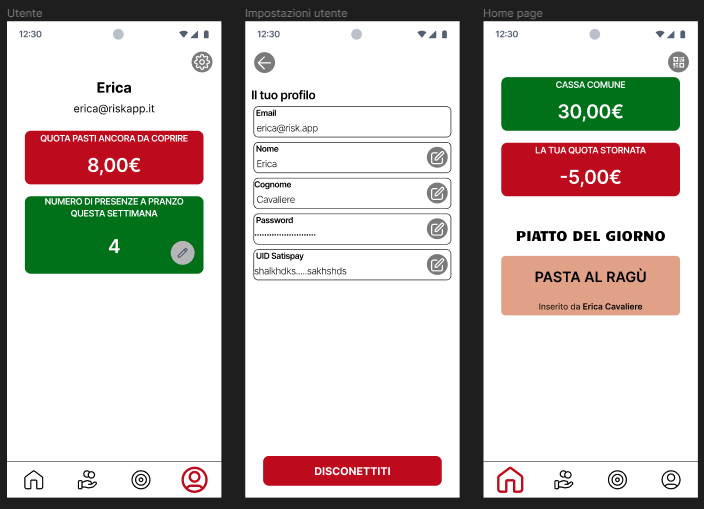
\includegraphics[width=0.9\columnwidth]{figma/esempi} 
    \caption{Alcune schermate progettate in Figma}
    \label{fig:schermatefigma}
\end{figure}
La schermata \textbf{Impostazioni} è raggiungibile attraverso la schermata \textbf{Utente}, andando a toccare l'icona ad ingranaggio posta nella barra superiore.\newline
Da \textbf{Impostazioni} è possibile modificare i dati dell'utente oppure permettere all'utente di disconnettersi dalla sessione corrente.\newline
\newline
Sono state create diversamente anche le finestre \textbf{Accedi} (Figura \ref{fig:accedifigma}) e \textbf{Registrati} (Figura \ref{fig:registratifigma}).\newline
In queste due schermate non sono presenti barre superiori o inferiori, ma solo una serie di campi da compilare e il pulsante verde Accedi o Registrati.\newline
\textbf{Accedi} è la prima schermata che vede l'utente quando entra nell'app per la prima volta; per passare alla schermata \textbf{Registrati} bisogna toccare il link presente sotto al pulsante Accedi, dove è scritto il messaggio "\emph{Sei nuovo? REGISTRATI}".\newline
Per ritornare alla schermata \textbf{Accedi}, il procedimento è analogo, ovvero si tocca il link presente sotto il pulsante Registrati, dove è riportato il messaggio "\emph{Hai già un account? ACCEDI}".\newline
Invece, per andare in \textbf{Home}, bisognerà compilare correttamente i campi e poi toccare il pulsante verde presente.\newline
\newline
In \textbf{Accedi} è presente il messaggio "\emph{Hai dimenticato la password?}", questo doveva contenere un link che permetteva all'utente di recuperare la propria password, funzionalità prima prevista, poi ritenuta non più necessaria.\newline
%qui poi si dovrà riportare le schermate a 0.7 in base all'introduzione ---------------------------------------------------------------------------------------------------------------------------------------------------------------------
\begin{figure}[!h] 
    \centering 
    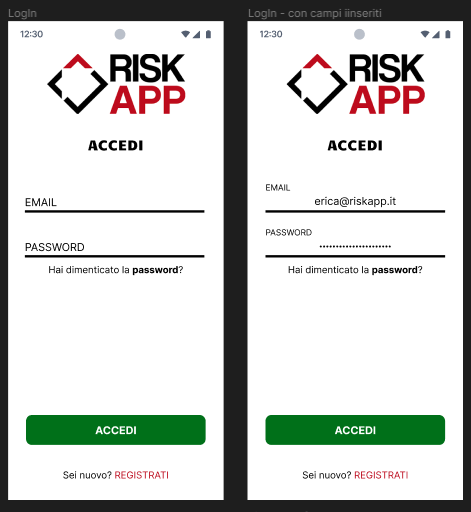
\includegraphics[width=0.6\columnwidth]{figma/accedi} 
    \caption{Schermata Accedi progettata in Figma}
    \label{fig:accedifigma}
\end{figure}
\begin{figure}[!h] 
    \centering 
    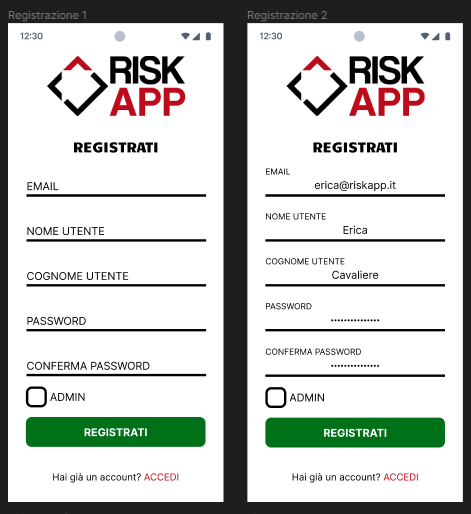
\includegraphics[width=0.6\columnwidth]{figma/registrati} 
    \caption{Schermata Registrati progettata in Figma}
    \label{fig:registratifigma}
\end{figure}
%Come è già stato detto, sono state fatte diverse modifiche in fase di progettazione, alcune modifiche sono state fatte perchè non rispettavano le idee del proponente, altre perchè non avevano utilità, come il recupero password appena accennato, altre modifiche sono state fatte anche a livello grafico, perchè non permetteva all'utente di capire che cosa poteva fare.\newline
%Per questo sono state fatte delle modifiche anche ai componenti utilizzati (nella figura \ref{fig:conteinerfigma} ci sono i \emph{component} creati per il \emph{mockup}), pure le icone dei pulsanti, che servivano solo a livello dimostrativo.
%\begin{figure}[!h] 
%    \centering 
%    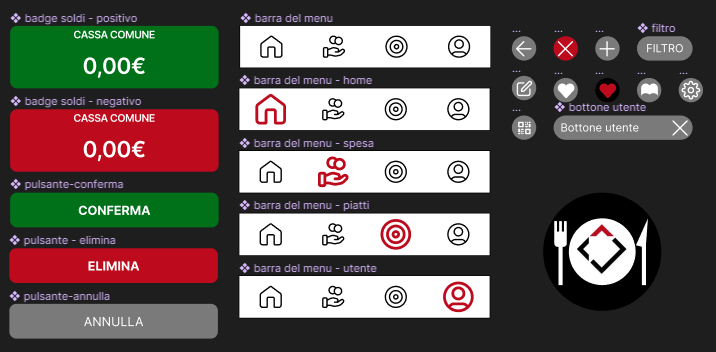
\includegraphics[width=0.9\columnwidth]{figma/container} 
%    \caption{Alcuni pulsati e icone progettate in Figma}
%    \label{fig:conteinerfigma}
%\end{figure}

\newpage

\subsection{Database}
Per quanto riguarda la base di dati (Figura \ref{fig:database}), ho pensato a una struttura semplice, mettendo al centro l'utente che può inserire dei piatti, delle transazioni oppure segnare le proprie presenze.\newline
Si è poi pensato ad un'entità isolata, che ha il solo scopo di contenere le variabili globali, ovvero la \emph{\gls{cassacomuneg}}, la \emph{\gls{quotapastog}} e la \emph{\gls{quotastornatag}} degli stagisti.\newline
Per quanto riguarda gli stagisti, inizialmente si pensava se considerarli come un utente oppure se rappresentarli come un'altra entità; alla fine, è stato deciso di lavorare in modo diverso, dato che gli stagisti si ipotizza che non utilizzino l'app.\newline
Gli utenti amministratori possono aggiungere le spese e le presenze degli stagisti, mentre la loro \emph{\gls{quotastornatag}} è stato deciso di indicarla nell'entità Cassa Comune, dato che si tratta di un dato unico per tutti gli stagisti.\newline
\begin{figure}[!h] 
    \centering 
    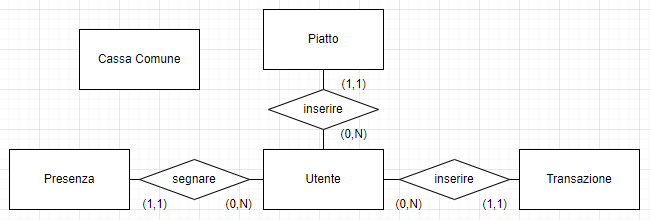
\includegraphics[width=0.9\columnwidth]{database} 
    \caption{Il database progettato per l'applicazione}
    \label{fig:database}
\end{figure}
\newline
Lavorando con Firebase, un database NoSQL, i dati sono stati gestiti in modo leggermente diverso, ma rimanendo fedeli alle entità riportate in Figura \ref{fig:database}.\newline
Questo perchè Firebase organizza i dati in \emph{raccolte}, ogni raccolta contiene dei \emph{documenti} e ogni documento è composto da \emph{campi}.\newline
Se dovessimo tradurre a livello teorico:
\begin{itemize}
    \item le \emph{raccolte} sono le entità;
    \item i \emph{documenti} sono le \emph{tuple}, cioè se dovessimo rappresentare le entità come una tabella, un documento è una riga di informazioni dell'entità;
    \item i \emph{campi} sono gli attributi, ovvero un singolo dato della \emph{tupla}.
\end{itemize}
Con Firebase si possono gestire i dati in modo diverso da quanto descritto, perchè i \emph{documenti} non sono rigidi, cioè i \emph{documenti} all'interno di una \emph{raccolta} possono avere quantità e tipi diversi di \emph{campi}, permettendo una struttura dinamica e lasciando al programmatore la libertà di decidere come gestire le informazioni.\newline
\newline
Per convenzione, è stato deciso di strutturare i dati come è stato descritto nell'elenco puntato, perchè risultava più semplice capire l'ordine delle informazioni e ha permesso una semplice gestione dei dati a livello di codice.\newline
Di seguito si riporta la struttura finale del database, riportando per ogni \textbf{raccolta} i \emph{campi} che ogni documento deve contenere.\newline

\newpage

\textbf{cassaComune}
\begin{itemize}
    \item \emph{cassaComune}, di tipo number (numerico)
    \item \emph{quotaPasti}, di tipo number
    \item \emph{quotaStornataStagisti}, di tipo number
\end{itemize}
Per questa raccolta esiste un solo \emph{documento} con codice identificativo "cassaComune".\newline

\textbf{utenti}
\begin{itemize}
    \item \emph{email}, di tipo string (stringa)
    \item \emph{nome}, di tipo string
    \item \emph{cognome}, di tipo string
    \item \emph{UID}, di tipo string; questo rappresenta il codice UID Satispay dell'utente
    \item \emph{quotaStornta}, di tipo string
    \item \emph{admin}, di tipo boolean (booleano)
\end{itemize}

\textbf{piatti}
\begin{itemize}
    \item \emph{nome}, di tipo string
    \item \emph{ingredienti}, di tipo string
    \item \emph{ricetta}, di tipo string
    \item \emph{propostoOggi}, di tipo timestamp; questo permette di capire quando è stata l'ultima volta che il piatto è stato proposto; se riporta la data odierna, il piatto dovrà comparire nella Home
    \item \emph{utente}, di tipo string; serve per capire quale utente ha inserito il piatto
\end{itemize}

\textbf{presenze}
\begin{itemize}
    \item \emph{data}, di tipo timestamp
    \item \emph{utente}, di tipo string
    \item \emph{quotaPasto}, di tipo number; indica quanto riportava la \emph{\gls{quotapastog}} il giorno in cui l'utente è stato presente a pranzo
    \item \emph{stagisti}, di tipo boolean; se impostato a \emph{true} vuol dire che la presenza indicata riporta la presenza degli stagisti e non dell'utente
    \item \emph{numStagisti}, di tipo number; se \emph{stagisti} è impostato a \emph{true} riporta quanti stagisti erano presenti nella data indicata
\end{itemize}
\newpage
\textbf{transazioni}
\begin{itemize}
    \item \emph{soldi}, di tipo number
    \item \emph{data}, di tipo timestamp
    \item \emph{utente}, di tipo sting
    \item \emph{stagista}, di tipo boolean; indica se è stato lo stagista ad effettuare la spesa (\emph{true}) o l'utente (\emph{false})
    \item \emph{spesa}, di tipo boolean; se \emph{true} indica che la transazione riportata è una spesa, altrimenti si tratta dell'invio dei soldi ad un altro utente
    \item \emph{utenteRiceveInvioSoldi}, di tipo string; se \emph{spesa} è impostato a \emph{false}, questo riporta l'utente che riceve i soldi
\end{itemize}

%\newpage

%\section{Design Pattern utilizzati}
%forse parlare dell'MVVM o BLoC patttern

\section{Codifica} %riportare qui il database?
%In questa sezione riporto la struttura della cartella lib, parlerò delle componenti e, del file firebase_option e delle classi
%riportare anche le immagine dell'app creata

\subsection{Struttura delle cartelle}
Per il progetto è stato installato il \emph{\gls{sdk}}\glsfirstoccur di Flutter nella versione 3.13.6.\newline  
%\newline
\begin{figure}[!h] 
    \centering 
    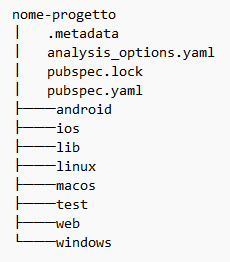
\includegraphics[width=0.35\columnwidth]{FlutterStructure} 
    \caption{La struttura del progetto preimpostata da Flutter}
    \label{fig:directory-flutter}
\end{figure}

La prima cosa che si nota quando si crea un progetto Flutter, è la struttura preimpostata dal \emph{framework} (Figura \ref{fig:directory-flutter}):
\begin{itemize}
    \item all'interno del file \emph{.metadata} si trovano le proprietà del codice Flutter; questo file \textbf{non} bisogna modificarlo perchè contiene i metadati del progetto;
    \item il file \emph{analysis\textunderscore options.yaml} serve per analizzare il codice Dart e controllare che non ci siano errori quando si compila il codice; come è intuibile, anche questo file \textbf{non} bisogna toccarlo;
    \item il file principale che controlla le librerie da installare è \emph{pubspec.yaml}; se si desidera aggiungere un pacchetto, impostare un font specifico o anche indicare la cartella dove bisogna reperire i video e le immagini, bisogna indicarli dentro a questo file;
    \item per ogni piattaforma (Android, iOS, Linux, MacOS, Web e Windows), è presente una cartella apposita con all'interno tutto l'occorrente per far funzionare il progetto nel sistema operativo desiderato;
    \item il codice principale lo si scrive all'interno della cartella \emph{lib};
    \item Flutter preimposta la cartella \emph{test} dove poter svolgere i test di unità.
\end{itemize}
Per questo progetto, ho lavorato principalmente nella cartella \emph{lib} e ho creato una cartella \emph{assets} per inserire il logo dell'azienda RiskAPP, visibile nella pagine Accedi e Registrati dell'app (se fossero state presenti altre immagini, sarebbero state inserite all'interno di questa cartella).\newline
Poche volte ho toccato le cartelle \emph{android} e \emph{ios}, principalmente per sistemare qualche libreria di Flutter che dava problemi su uno dei due sistemi operativi. 
%\newpage
\begin{figure}[!h] 
    \centering 
    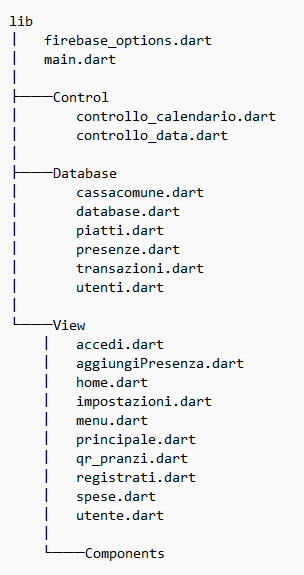
\includegraphics[width=0.45\columnwidth]{libDirectory} 
    \caption{La struttura della cartella lib}
    \label{fig:directory-lib}
\end{figure}

Come si può vedere in Figura \ref{fig:directory-lib}, ho creato tre cartelle per suddividere i file:
\begin{itemize}
    \item nella cartella \textbf{Control}, sono state definite le classi per poter gestire le variabili locali dell'app, che sono solo di supporto per poter gestire alcune informazioni, come per esempio impostare la data nel formato italiano, implementato nella classe ControlloData() creata nel file \emph{controllo\textunderscore  data.dart};
    \item all'interno di \textbf{Database}, sono presenti tutte le classi con le funzioni appropriate per poter comunicare e gestire il database di Firebase;
    \item all'interno della cartella \textbf{View}, viene gestita la parte grafica dell'app; per ogni pagina è stata creato un file apposito, l'unica eccezione è per \emph{principale.dart} che ha il solo scopo di visualizzare la barra inferiore dell'app.
\end{itemize}
Il file \emph{firebase\textunderscore options.dart} contiene le istruzioni fondamentali per collegare il progetto alla console di Firebase e viene generato automaticamente da \emph{FlutterFire \gls{clig}\glsfirstoccur}, un tool che mette a disposizione diversi comandi per installare \emph{FlutterFire} e permettere di collegare il proprio progetto a Firebase.\newline
In \emph{main.dart} si decide quale pagina deve visualizzare l'utente quando apre l'app, in base se è stato eseguito l'accesso le volte precedenti o no.
%\newpage
\begin{figure}[!h] 
    \centering 
    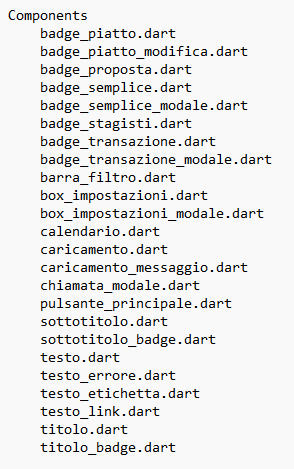
\includegraphics[width=0.45 \columnwidth]{ComponentsDirectory} 
    \caption{La struttura della cartella Components}
    \label{fig:directory-components}
\end{figure}

In \textbf{View} è presente la cartella \textbf{Components} (Figura \ref{fig:directory-components}), questa contiene le componenti, ovvero degli elementi preimpostati che vengono utilizzati più volte all'interno del codice.\newline
Per esempio, il file \emph{caricamento.dart} definisce la schermata che dovrà essere visibile mentre viene eseguito un caricamento dei dati da Firebase; questo componente viene richiamato da quasi tutte le pagine create in \textbf{View}.

\newpage

\subsection{Le librerie di Firebase}
Quando si collega un progetto a Firebase, si scaricano i pacchetti \emph{Firebase \gls{clig}} e \emph{FlutterFire \gls{clig}}, questi permettono di collegare il progetto alla console di Firebase e creano il file \emph{firebase\textunderscore option.dart} che dovrà poi essere importato nel file \emph{main.dart}.\newline
Infine, basta scrivere le righe di codice riporte in Figura \ref{fig:code-firebase} per poter permettere ad ogni piattaforma di interagire con il database.
\begin{figure}[!h] 
    \centering 
    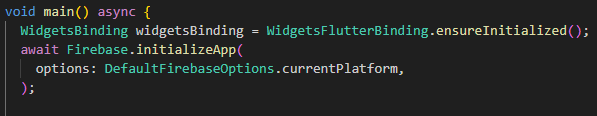
\includegraphics[width=0.95 \columnwidth]{code/firebase} 
    \caption{Istruzioni per collegare Firebase}
    \label{fig:code-firebase}
\end{figure}

Quando si eseguono i passaggi appena descritti, si installa in automatico il pacchetto \emph{firebase\textunderscore core}, ma per poter permettere l'autenticazione degli utenti e lavorare con il database, sono stati installati manualmente i pacchetti \emph{firebase\textunderscore auth} e \emph{cloud\textunderscore firestore}.\newline
\newline
Ci sono diversi modi che Firebase Authentication mette a disposizione per la registrazione di un utente, ma per questo progetto è stato adottato il metodo di autenticazione tramite mail e password.\newline
Per permettere la registrazione, l'accesso e la disconnessione di un utente, è stato creata la classe \emph{Database} che al suo interno contiene solo i metodi con le funzioni appena descritte (in Figura \ref{fig:code-authentication} sono riportate le funzioni \emph{accedi} e \emph{disconettiti}).
\begin{figure}[!h] 
    \centering 
    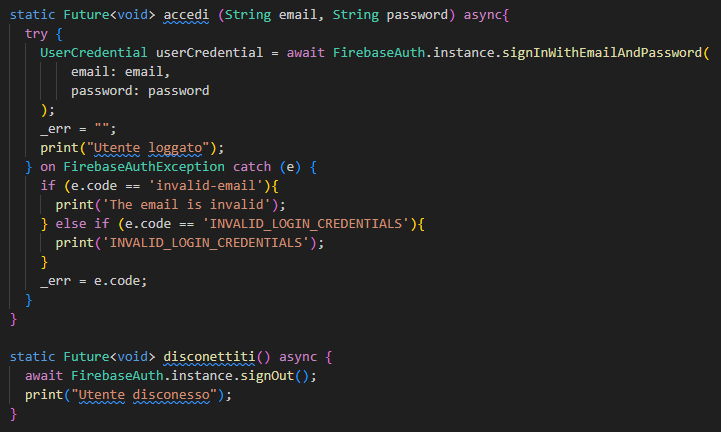
\includegraphics[width=1.05 \columnwidth]{code/firebaseauth} 
    \caption{Le funzioni di accesso e di disconnessione di un utente}
    \label{fig:code-authentication}
\end{figure}

\newpage

Per poter lavorare con il Cloud di Firestore, è stata creata una classe per ogni entità.\newline
Ogni classe contiene un metodo per creare una nuova istanza (Figura \ref{fig:code-aggiungi}), metodi \emph{set} e \emph{get} per ogni campo (Figura \ref{fig:code-query}) e alcune funzioni di supporto.
\begin{figure}[!h] 
    \centering 
    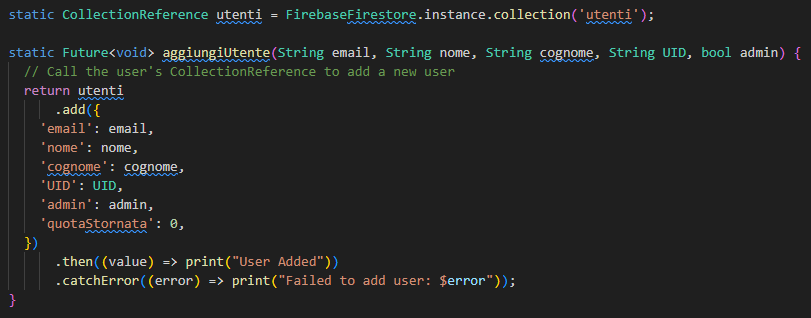
\includegraphics[width=1.1 \columnwidth]{code/aggiuntautente} 
    \caption{La funzione di aggiunta di un utente nel database}
    \label{fig:code-aggiungi}
\end{figure}
\begin{figure}[!h] 
    \centering 
    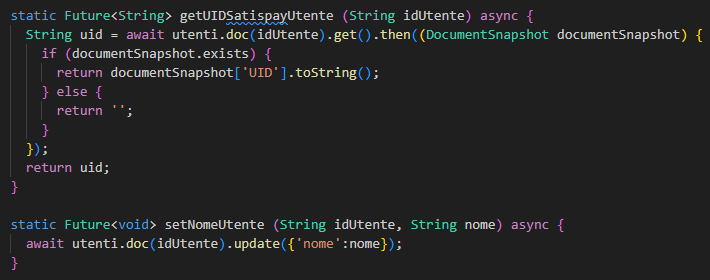
\includegraphics[width=1.00 \columnwidth]{code/query-set} 
    \caption{Una funzione \emph{get} e \emph{set} della classe \emph{Utenti}}
    \label{fig:code-query}
\end{figure}

Attraverso la console di Firebase è possibile vedere gli utenti che si sono registrati, i dati presenti nel database ed è possibile anche modificare i permessi di lettura o modifica dei dati, per un controllo più attento anche a livello di codice. 

\newpage

\subsection{Il calendario delle presenze}
Per permettere la gestione delle presenze, è stato installato il pacchetto \emph{table\textunderscore calendar}, che permette di creare il \emph{widget} TableCalendar, cioè l'elemento grafico che vediamo in Figura \ref{fig:calendario}.
\begin{figure}[!h] 
    \centering 
    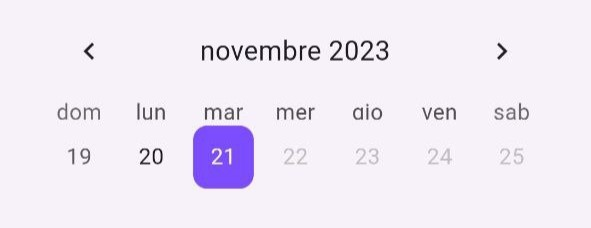
\includegraphics[width=0.5 \columnwidth]{calendario} 
    \caption{Il calendario che l'utente utilizza per gestire le presenze}
    \label{fig:calendario}
\end{figure}

Il \emph{widget} offre una serie di opzioni che consentono di modificarlo, come per esempio scegliere se visualizzare il calendario nel formato settimanale (come in immagine), con due settimane oppure tutto un mese.\newline
Si può modificare come viene visualizzata la data selezionata (anche la data odierna) attraverso l'uso del \emph{CalendarBuilder}: si tratta di un costruttore (\emph{builder}) con il compito di impostare la grafica dell'elemento indicato; in questo caso ha il compito di impostare la grafica delle date evidenziate.\newline
\newline
Questo calendario è presente nella pagina Utente, dove sono visibili i tre \emph{widget} grigi, il primo apre il calendario per modificare le proprie presenze (Figura \ref{fig:utente-presenze}), il secondo, visibile per gli amministratori, apre il calendario per modificare e monitorare le presenze degli stagisti.\newline
Il terzo \emph{widget} consente solo di visualizzare e modificare la \emph{\gls{quotapastog}}.\newline
Non sono stati inseriti altri calendari nell'applicazione.\newline
\newline
Una funzione fondamentale di TableCalendar è \emph{onDaySelected}: questa permette di modificare il calendario selezionato, rendendo la selezione iterativa; se non viene definita questa funzione, il calendario rimane statico e non sarà possibile cambiare la data selezionata, ma rimarrà evidenziata la data indicata inizialmente nella variabile \emph{focusedDay}.
\newpage
\begin{figure}[!h] 
    \centering 
    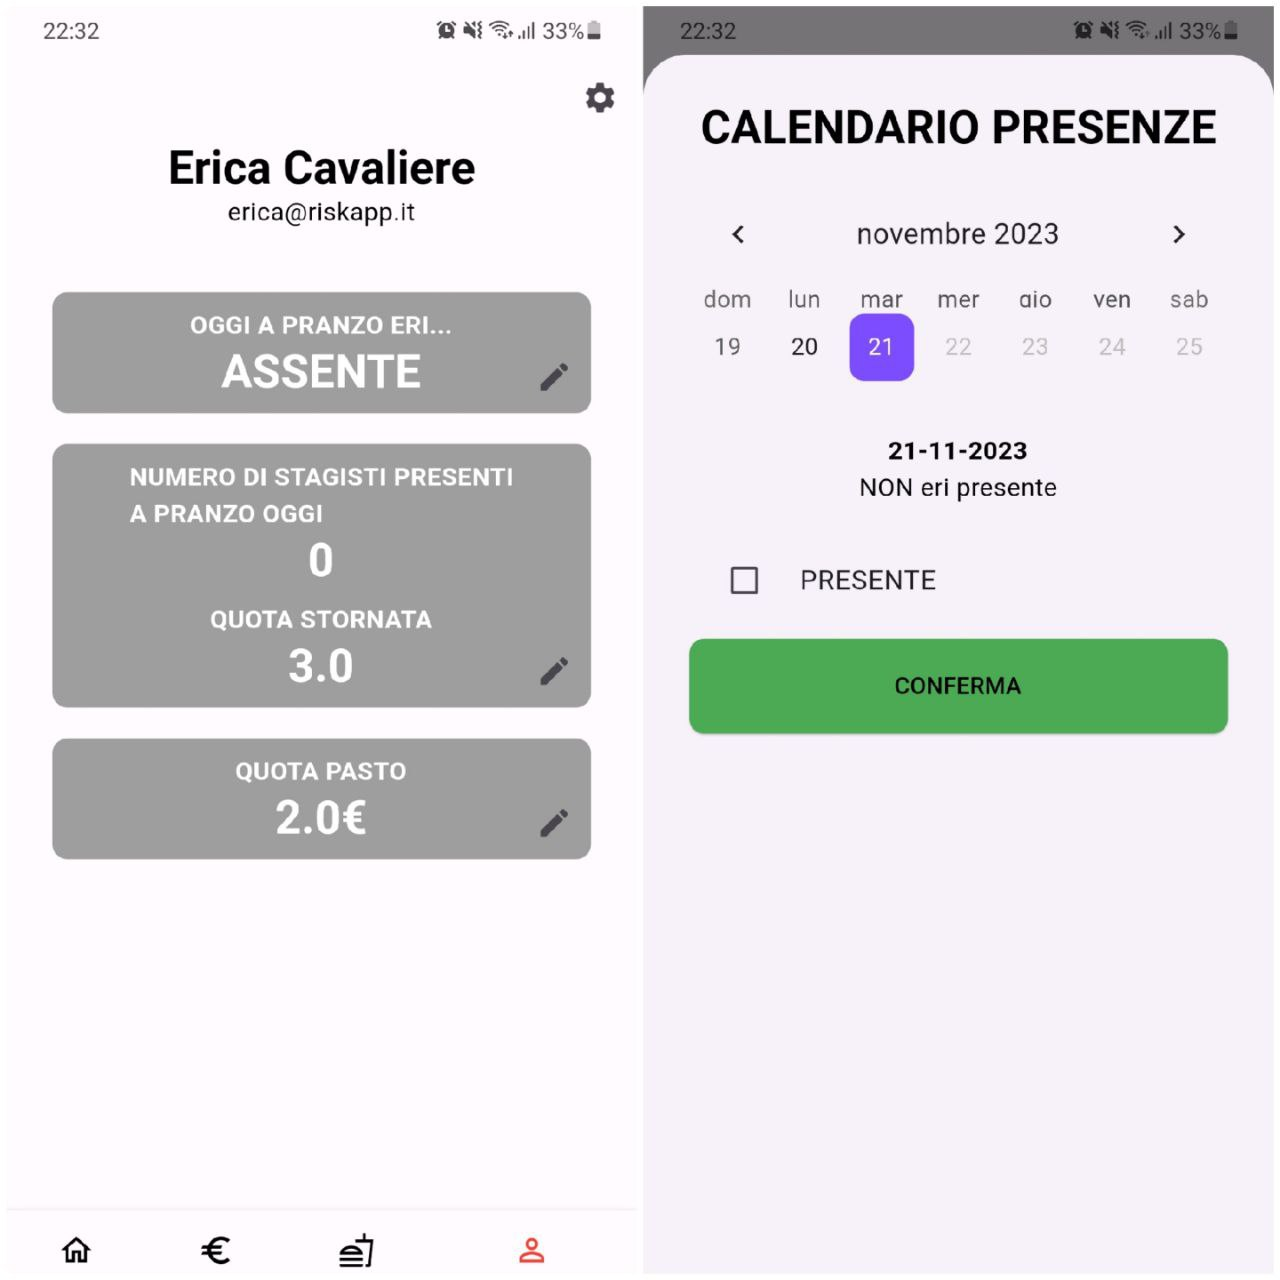
\includegraphics[width=0.7 \columnwidth]{Utente} 
    \caption{La schermata Utente e il calendario delle presenze}
    \label{fig:utente-presenze}
\end{figure}
\begin{figure}[!h] 
    \centering 
    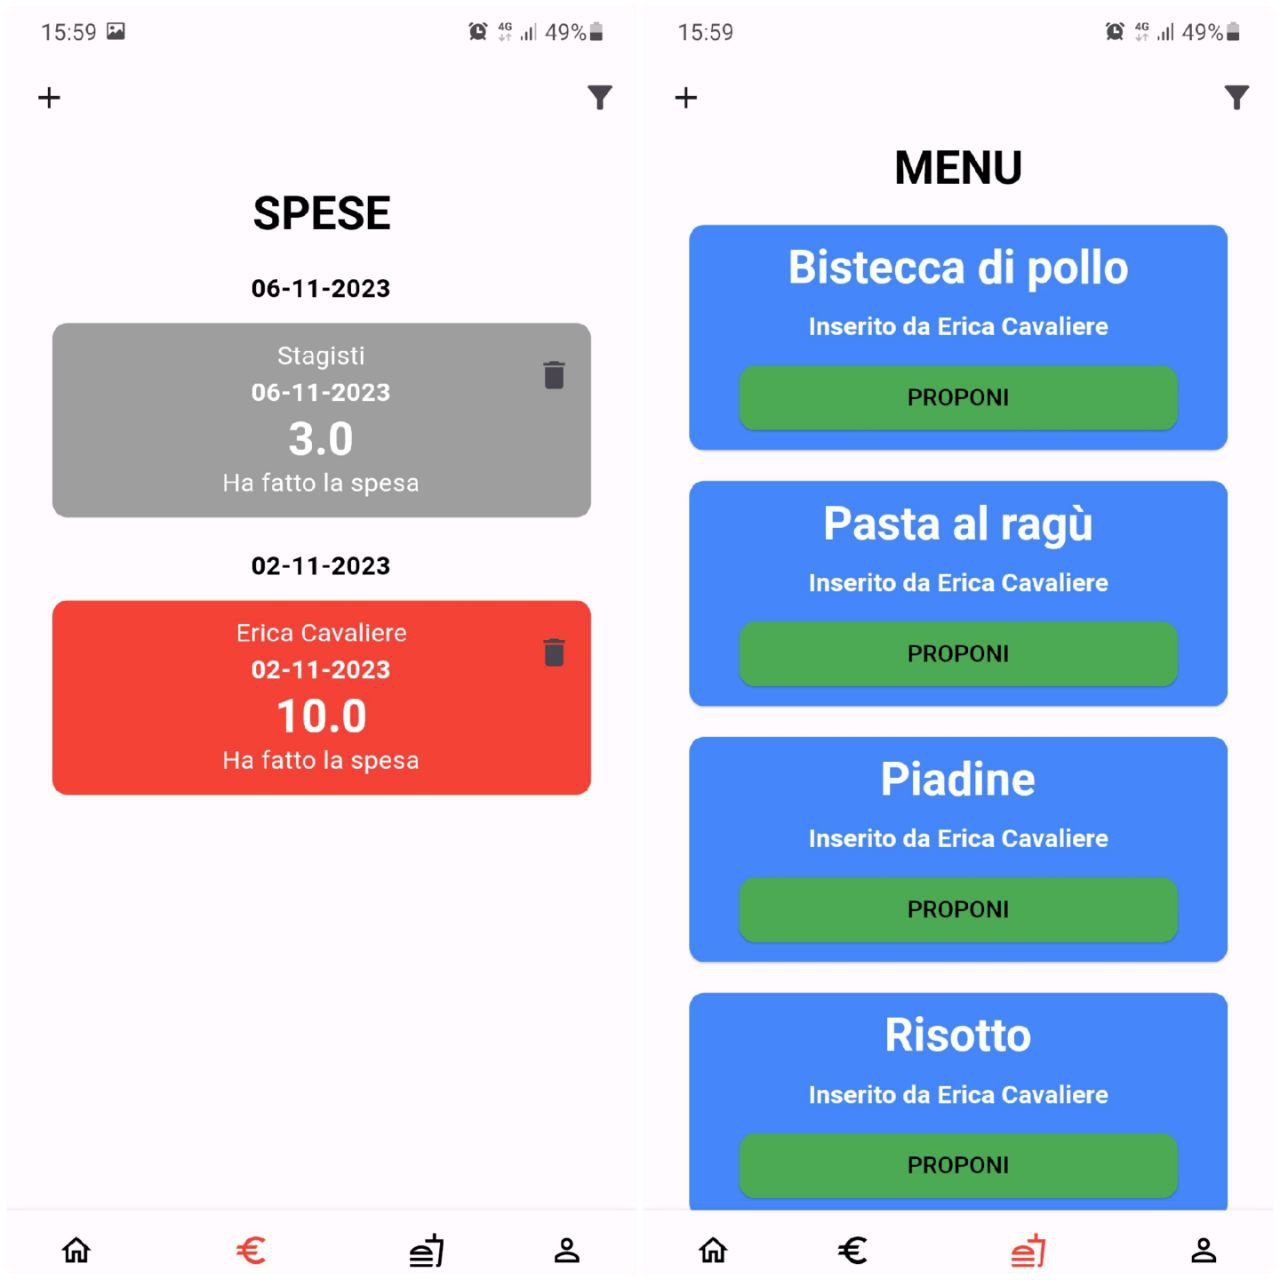
\includegraphics[width=0.7 \columnwidth]{SpeseMenu} 
    \caption{Le schermate Spese e Menu}
    \label{fig:spese-menu}
\end{figure}
\newpage

\subsection{Altre schermate dell'app}
Per questo progetto è stata richiesta un'app che permettesse, oltre un controllo e una gestione delle presenze, anche un controllo delle spese e la presenza di un menu comune per tutti, dove è possibile proporre un piatto per il pranzo odierno (Figura \ref{fig:spese-menu}).\newline
Tramite la barra superiore di entrambe le schermate, è possibile aggiungere un elemento alla lista oppure utilizzare il filtro per visualizzare solo alcuni elementi specifici.\newline
\newline
Quando si effettua una aggiunta o si applica un filtro, il lavoro che l'app svolge è aggiornare il database o richiedere degli elementi specifici nel cloud di Firebase, per poi aggiornare graficamente la lista interessata.\newline
Ogni modifica in Firebase viene ripotata in tempo reale su tutti i dispositivi che utilizzano l'app; per permettere questo, sono stati utilizzati gli \textbf{StreamBuilder} (\cite{site:flutter-streambuilder}).\newline
Dato uno \emph{stream} di dati, lo \textbf{StreamBuilder} si occupa di creare e aggiornare dei \emph{widget} specifici, in questo caso si occupa di aggiornare le liste presenti nelle schermate Spesa e Menu.\newline
\newline
Lo \textbf{StreamBuilder} è stato utilizzato anche nella Home, per permettere all'utente di monitorare in tempo reale i piatti proposti, la \emph{\gls{cassacomuneg}} e la propria \emph{\gls{quotastornatag}}, quest'ultimi due sono in continuo aggiornamento in base alle modifiche riportate nella schermata Spese o tramite le presenze segnate nel calendario (per ogni presenza viene effettuata una modifica pari alla quantità di soldi indicata nella \emph{\gls{quotapastog}}).\newline
È stato utilizzato lo \textbf{StreamBuilder} anche nella schermata Utente per il controllo in tempo reale della \emph{\gls{quotastornatag}} degli stagisti.

%\newpage

\subsection{Modificare il nome e il logo}
Quando si crea un'applicazione, di default Flutter imposta il suo logo.\newline
Per poter modificare e utilizzare il proprio logo è molto semplice, prima di tutto bisogna creare più formati dell'immagine che si desidera attribuire all'app, poi bisogna riportarli tutti all'interno della cartella del sistema operativo interessato e preimpostato da Flutter.
\begin{itemize}
    \item Per Android bisogna salvare il logo e tutti i suoi formati nel percorso\newline \emph{android/app/src/main/res}
    \item Per iOS bisogna salvare il logo e tutti i suoi formati nel percorso\newline \emph{ios/Runner/Assets.xcassets/AppIcon.appiconset}
\end{itemize}
Il logo per questo progetto è stato creato in Figma (Figura \ref{fig:logo-nome}).\newline
\newline
Il procedimento per modificare il nome dell'applicazione non si discosta molto dal procedimento appena descritto.
\begin{itemize}
    \item Per Android bisogna modificare il parametro \emph{label} presente nel file\newline \emph{AndroidManifest.xml} che si trova nel percorso \emph{android/app/src/main}.
    \item Per iOS bisogna modificare il parametro \emph{CFBundleDisplayName} nel file \emph{Info.plist} presente nel percorso \emph{ios/Runner}.
\end{itemize}
\begin{figure}[!h] 
    \centering 
    
\includegraphics[width=0.2 \columnwidth]{GestionePranzi} 
    \caption{Il nome e il logo dell'applicazione creata}
    \label{fig:logo-nome}
\end{figure}

%\newpage

\subsection{Aprire l'app tramite QrCode}
Per poter gestire le presenze in modo veloce, si pensava di utilizzare un QrCode che permettesse di segnare la presenza dell'utente quando veniva scannerizzato.\newline
Purtroppo, non è stato possibile implementare questa funzione perchè sono state incontrate diverse difficoltà nel creare quanto richiesto, ma è stato un caso di studio interessante che potrebbe essere approfondito in futuro.\newline
\newline
Per poter creare un qualsiasi QrCode, è stato installato il pacchetto \emph{qr\textunderscore flutter}; quest'ultimo permette di creare il \emph{widget QrImageView}, che si occupa di far vedere direttamente nell'applicazione un QrCode, generato da una stringa impostata dal programmatore.\newline
Il dubbio a questo punto sorge spontaneo: se bisogna passare una parola, una frase, un qualsiasi testo per creare un QrCode, qual è la stringa che permette di aprire la propria applicazione Flutter?\newline
La risposta, in realtà, è molto semplice a parole, ma nella pratica incontra qualche difficoltà.\newline
Per aprire un'applicazione, bisogna creare un URL identificativo per l'app e questa sarà la stringa che bisognerà passare a \emph{QrImageView} per generare il QrCode desiderato.\newline
\newline
Creare un URL è molto semplice, ci sono diversi servizi online che permettono di creare il proprio sito e ottenere così un indirizzo web.\newline
In accordo con il mio tutor, è stato scelto di utilizzare il servizio Hosting di Firebase; il passaggio successivo consiste nel collegare il proprio progetto Flutter all'URL creato.\newline
\newline
Per configurare correttamente la propria app Flutter, bisogna utilizzare la navigazione tramite \emph{route}, ovvero associando un percorso per ogni pagina che si desidera aprire, oppure installando la libreria \emph{go\textunderscore route}.\newline
Questo è stato il mio primo errore per testare il QrCode, perchè per gestire la navigazione tra pagine, ho utilizzato il \emph{widget Navigator}; per questo motivo è stata installata successivamente la libreria richiesta e ho creato un file di test, ovvero una schermata contenente un messaggio di conferma presenza.\newline
\newline
Dopo aver configurato il percorso di ogni schermata, bisogna modificare il file \emph{AndroidManifest.xml} per Android e il file \emph{Info.plist} per iOS, aggiungendo delle istruzioni specifiche che permettono la navigazione tramite i \textbf{Deep Link}.\newline
\newline
I \textbf{Deep Link} sono un modo semplice per connettere le pagine di un'app.\newline
Con questo metodo è possibile collegare la propria app ad altre, ma anche direzionare gli utenti a specifiche pagine in-app.\newline
Questa tecnologia aiuta l’ecosistema mobile a diventare più connesso, piuttosto che creare una serie di applicazioni che non possono “comunicare” tra di loro.\newline
Da non confondere con i \textbf{Dynamic link}, che sono sempre dei \textbf{Deep Link}, ma permettono di personalizzare il comportamento di questi.\newline
Ad esempio, lo stesso link può portare ad una determinata sezione dell'app per Android ma ad una diversa sezione dell'app per iOS oppure, se l'utente non ha l'app installata, può spedirlo allo store (di Google, o di Apple) per scaricare l'applicazione.\newline
Dopo l'installazione il link porta a termine il suo compito aprendo la sezione giusta dell'app oppure, se preferiamo, possiamo chiedere al link di inviare al nostro sito Web l'utente che non ha l'app installata sul suo smartphone.\newline
\newline
Dopo aver configurato la propria applicazione, creato l'URL e connesso l'app al sito, ora è possibile creare un QrCode che permette di aprire direttamente l'applicazione o, se l'app non è installata, aprire la pagina web.\newline
Questo è tutto quello che sono riuscita a fare, ho seguito tutti i passaggi appena descritti, creato il QrCode passando come stringa l'URL dell'app e, se si scannerizza il QrCode con un qualsiasi lettore di codici Qr, aprire l'applicazione.\newline
\newline
Considerando quanto fatto, possiamo definirlo un successo, perchè sono riuscita a studiare e a fare una cosa per me nuova, ma non una vittoria, perchè il QrCode non doveva solo aprire l'applicazione, doveva anche direzionare l'utente ad una pagina specifica e permettere così di segnare la propria presenza a pranzo nella giornata odierna.\newline
Per questo ultimo passaggio sono state incontrate diverse difficoltà, decidendo così di abbandonare l'idea, dato che è già possibile segnare manualmente la propria presenza tramite il calendario, ma sarà una sfida che affronterò ancora in futuro.

    \chapter{Verifica e validazione}
\label{cap:verifica-validazione}

    \chapter{Conclusioni}
\label{cap:conclusioni}

\intro{In conclusione a tutto il percorso di stage, questo capitolo riporta un resoconto degli obiettivi e dei requisiti raggiunti, seguito poi da un'analisi personale del progetto svolto.}\\ 

\section{Raggiungimento degli obiettivi}
In riferimento alle notazioni indicate nel \hyperref[sec:obbiettivi]{primo capitolo} e nel \hyperref[sec:requisiti]{terzo capitolo} e in riferimento alle Tabelle \ref{tab:obiettivi-richiesti}, \ref{tab:requisiti-funzionaliuno}, \ref{tab:requisiti-funzionalidue}, \ref{tab:requisiti-qualitativi} e \ref{tab:requisiti-vincolo}, di seguito sono riportati gli obbiettivi e i requisiti con il loro stato di completamento.\newline
Alcuni obbiettivi e alcuni requisiti non sono stati soddisfatti perchè è stato deciso di impiegare più tempo per il raggiungimento degli obiettivi obbligatori, dedicando più tempo allo studio e cercando di migliorare alcune funzioni dell'applicazione richiesta.\newline

\subsection{Obiettivi raggiunti}
%Si farà riferimento ai requisiti secondo le seguenti notazioni:
%\begin{itemize}
%    \item O per i requisiti obbligatori, vincolanti in quanto obiettivo primario richiesto dal committente;
%    \item D per i requisiti desiderabili, non vincolanti o strettamente necessari, ma dal riconoscibile valore aggiunto;
%    \item F per i requisiti facoltativi, rappresentanti valore aggiunto non strettamente competitivo.
%\end{itemize}
%Le sigle precedentemente indicate saranno seguite da una coppia sequenziale di numeri, identificativo del requisito.

\begin{table}[htb]%
    \caption{Tabella degli obiettivi raggiunti}
    \label{tab:obiettivi-raggiunti}
    \begin{tabularx}{\textwidth}{lXl}
    \hline
    \textbf{Obiettivo} & \textbf{Descrizione} & \textbf{Stato}\\
    \hline\hline
    O01     & Accesso tramite credenziali & Soddisfatto \\
    \hline
    O02     & Pannello di controllo degli utenti & Soddisfatto \\
    \hline
    O03     & Modifica o aggiunta delle spese & Soddisfatto \\
    \hline
    O04     & Monitoraggio della cassa comune & Soddisfatto \\
    \hline
    O05     & Controllo presenza in azienda di una persona durante i pranzi & Soddisfatto \\
    \hline
    O06     & Impostare il menu del giorno & Soddisfatto \\
    \hline
    O07     & Scelta di un piatto dal menu & Soddisfatto \\
    \hline
    D01     & Integrazione di ChatGPT per consigliare alcune ricette & Non soddisfatto \\
    \hline
    F01     & Test a livello di frontend & Non soddisfatto \\
    \hline
    \end{tabularx}
\end{table}%

\newpage

\subsection{Requisiti funzionali raggiunti}

\begin{table}[htb]%
\caption{Tabella del tracciamento dei requisiti funzionali dall'1 al 17 raggiunti}
\label{tab:reqfunzionali-raggiunti}
\begin{tabularx}{\textwidth}{lXl}
\hline
\textbf{Requisito} & \textbf{Descrizione} & \textbf{Stato}\\
\hline\hline
RFO-1     & L'utente effettua l'accesso all'app inserendo la propria password e la propria mail & Soddisfatto \\
\hline
RFO-2     & L'utente si registra nel database inserendo il proprio nome, cognome, mail e password & Soddisfatto\\
\hline
RFO-3     & Si visualizza la \emph{\gls{cassacomuneg}} salvata nel database nell'app & Soddisfatto \\
\hline
RFO-4     & L'utente visualizza la propria \emph{\gls{quotastornatag}} salvata nel database nell'app & Soddisfatto \\
\hline
RFO-5     & Si visualizza la lista dei piatti proposti del giorno nell'app & Soddisfatto \\
\hline
RFO-6     & Si visualizza la lista delle transazioni nell'app & Soddisfatto \\
\hline
RFO-7     & L'utente aggiunge una nuova transazione nell'app, indicando i soldi e la data e salva la transazione nel database & Soddisfatto \\
\hline
RFO-8     & L'utente amministratore aggiunge la spesa effettuata da uno stagista nell'app, indicando la data e quanto ha speso e lo salva nel database & Soddisfatto \\
\hline
RFO-9     & L'utente indica la spesa che ha effettuato nell'app, riportando i soldi e la data e lo salva nel database & Soddisfatto \\
\hline
RFO-10    & L'utente indica nell'app i soldi che ha inviato a un altro utente registrato nel database e salva la transazione nel database & Soddisfatto \\
\hline
RFO-11    & L'utente elimina una transazione presente nel database dall'app & Soddisfatto \\
\hline
RFO-12    & Si visualizza il menu che contiene la lista dei piatti dall'app & Soddisfatto \\
\hline
RFO-13    & L'utente aggiunge un nuovo piatto nell'app, indicando il nome del piatto, gli ingredienti e la ricetta e lo salva nel database & Soddisfatto \\
\hline
RFO-14    & L'utente elimina un piatto presente nel database dall'app & Soddisfatto \\
\hline
RFO-15    & L'utente propone un piatto da mangiare a pranzo selezionandolo dal menu & Soddisfatto \\
\hline
RFO-16    & L'amministratore visualizza la \emph{\gls{quotapastog}} dall'app & Soddisfatto \\
\hline
RFO-17    & L'amministratore modifica la \emph{\gls{quotapastog}} dall'app e salva il nuovo valore nel database & Soddisfatto \\
\hline
\end{tabularx}
\end{table}%

\begin{table}%
\caption{Tabella del tracciamento dei requisiti funzionali dal 18 al 35 raggiunti}
%\label{tab:requisiti-funzionali}
\begin{tabularx}{\textwidth}{lXl}
\hline
\textbf{Requisito} & \textbf{Descrizione} & \textbf{Stato}\\
\hline\hline
RFO-18    & L'amministratore visualizza la \emph{\gls{quotastornatag}} degli stagisti dall'app & Soddisfatto \\
\hline
RFO-19    & L'amministratore visualizza la lista con indicato i giorni di presenza degli stagisti dall'app & Soddisfatto \\
\hline
RFO-20    & L'amministratore modifica la lista con indicato i giorni di presenza degli stagisti dall'app e salva le modifiche nel database & Soddisfatto \\
\hline
RFO-21    & L'utente visualizza la lista con indicati i propri giorni di presenza a pranzo dall'app & Soddisfatto \\
\hline
RFO-22    & L'utente modifica la lista con indicati i propri giorni di presenza a pranzo dall'app e salva le modifiche nel database & Soddisfatto \\
\hline
RFO-23    & L'utente si disconnette dall'app & Soddisfatto \\
\hline
RFO-24    & L'utente visualizza i propri dati dall'app & Soddisfatto \\
\hline
RFO-25    & L'utente visualizza la propria mail dall'app & Soddisfatto \\
\hline
RFO-26    & L'utente visualizza il proprio nome dall'app & Soddisfatto \\
\hline
RFO-27    & L'utente visualizza il proprio cognome dall'app & Soddisfatto \\
\hline
RFO-28    & L'utente visualizza il proprio UID Satispay dall'app & Soddisfatto \\
\hline
RFO-29    & L'utente modifica i propri dati dall'app e salva le modifiche nel database & Soddisfatto \\
\hline
RFO-30    & L'utente modifica la propria password dall'app e salva la nuova password nel database & Soddisfatto \\
\hline
RFO-31    & L'utente modifica il proprio nome dall'app e salva il nuovo nome nel database & Soddisfatto \\
\hline
RFO-32    & L'utente modifica il proprio cognome dall'app e salva il nuovo cognome nel database & Soddisfatto \\
\hline
RFO-33    & L'utente modifica il proprio UID Satispay e salva il nuovo UID nel database & Soddisfatto \\
\hline
RFD-34    & Viene chiesto a ChatGPT una possibile ricetta da proporre a pranzo & Non soddisfatto \\
\hline
RFD-35    & Si aggiunge la ricetta proposta da ChatGPT nel menu e si salva la ricetta nel database & Non soddisfatto \\
\hline
\end{tabularx}
\end{table}%

\newpage

\subsection{Requisiti qualitativi raggiunti}

\begin{table}[htb]%
\caption{Tabella del tracciamento dei requisiti qualitativi raggiunti}
\label{tab:reqqualitativi-raggiunti}
\begin{tabularx}{\textwidth}{lXl}
\hline
\textbf{Requisito} & \textbf{Descrizione} & \textbf{Stato}\\
\hline\hline
RQN-1    & Il codice \emph{front-end} deve essere coperto da test di unità & Non soddisfatto \\
\hline
\end{tabularx}
\end{table}%

\subsection{Requisiti di vincolo raggiunti}

\begin{table}[htb]%
\caption{Tabella del tracciamento dei requisiti di vincolo raggiunti}
\label{tab:reqvincolo-raggiunti}
\begin{tabularx}{\textwidth}{lXl}
\hline
\textbf{Requisito} & \textbf{Descrizione} & \textbf{Stato}\\
\hline\hline
RVO-1    & L'applicazione deve essere sviluppato con il \emph{framework} Flutter & Soddisfatto \\
\hline
RVO-2    & L'applicazione deve essere sviluppato con la piattaforma Firebase & Soddisfatto \\
\hline
RVO-3    & L'applicazione deve essere accessibile su cellulari con sistema operativo Android e iOS & Soddisfatto \\
\hline
RVO-4    & La mail che l'utente deve utilizzare per registrarsi nel database e accedere all'app deve essere fornita da RiskAPP & Soddisfatto \\
\hline
RVO-5    & La mail dell'utente non deve essere modificabile tramite app & Soddisfatto \\
\hline
\end{tabularx}
\end{table}%

%\section{Conoscenze acquisite}

\section{Valutazione personale}
Considerando che ho affrontato questo progetto, partendo senza avere conoscenze di Flutter o di Firebase, posso dire di essere soddisfatta del lavoro svolto, perchè ho imparato e studiato qualcosa di nuovo.\newline
\newline
Non nego che ci sono state diverse difficoltà, in particolare con Firebase, perchè non riuscivo a capire come collegare la console Firestore e lavorare sul database tramite codice Dart, ma con calma, pazienza e diversi test e ricerche, sono riuscita a capire come implementare le funzioni utili per permettere un corretto funzionamento dell'app, rendendola usabile per tutti i dispositivi.\newline
\newline
Ho imparato Flutter, Firebase, ho capito quanto sia utile progettare il modello di un software tramite Figma, perchè avere una idea visiva del progetto da creare può aiutare a capire e a far capire su cosa si lavora e i relativi problemi da affrontare.\newline
\newline
Valutando il prodotto finale, ci sono molti punti che si possono migliorare, ma rispetta tutti gli obbiettivi e i requisiti obbligatori richiesti e l'azienda non ha trovato difficoltà nell'utilizzare l'applicazione creata.\newline


    \appendix
    \chapter{Appendice A}

\epigraph{Citazione}{Autore della citazione}


    \backmatter
    \printglossary[type=\acronymtype, title=Acronimi e abbreviazioni, toctitle=Acronimi e abbreviazioni]
    \printglossary[type=main, title=Glossario, toctitle=Glossario]

    \cleardoublepage
\chapter{Bibliografia}

\nocite{*}

% Print book bibliography
\printbibliography[heading=subbibliography,title={Riferimenti bibliografici},type=book]

% Print site bibliography
\printbibliography[heading=subbibliography,title={Siti web consultati},type=online]

\end{document}
